\section{Theorie}
\label{sec:Theorie}
In diesem Experiment soll die Energiedifferenz der Zeemannniveaus untersucht werden. Dazu wird das Verfahren des optischen Pumpens verwendet, was eine präzise Bestimmung ermöglicht.

Die Elektronen in einem Atom können nur diskrete Energien annehmen. Die Besetzungen $N_1$ und $N_2$  zweier Energielevel $W_1$ und $W_2$ (mit $W_1<W_2$) wird duch die Boltzmannverteilung beschrieben.
\begin{equation}
	\frac{N_2}{N_1}=\frac{g_2}{g_1}\frac{\exp(-W_2k_\mathrm{B}T)}{\exp(-W_1k_\mathrm{B}T)}
	\label{eqn:Bolztmann}
\end{equation}
Dabei ist $k_\mathrm{B}$ die Bolztmannkonstante, $T$ die Temperatur und $g_i$ die statistischen Gewichte. Das optische Pumpen ermöglicht es diese natürliche Verteilung so anzuregen, das $N_2 > N_1$ gilt. Mit einem induzierten Strahlenübergang kann dann die Energiedifferenz $W_2-W_1$ genau bestimmt werden.
\subsection{Magnetische Momente}
Da sowohl der Bahndrehimpuls $\vec{L}$ als auch der Spin $\vec{S}$ ein magnetisches Moment $\vec{\mu_L}$ bzw. $\vec{\mu_S}$ haben, hat auch die Kopplung $\vec{J}$ ein magnetisches Moment $\vec{\mu_J}$.
\begin{align}
	\vec{\mu_J}&=\vec{\mu_L} +\vec{\mu_S} & \left| \vec{\mu_J} \right|&=g_J\mu_B\left| \vec{J} \right|
\end{align}
Dabei präzediert $\vec{\mu_J}$ um $\vec{J}$, und über die Zeit gemittelt verschwinden die senkrechten Anteile.
Wenn ein äußeres Magnetfeld $B$ anliegt, präzediert $\vec{\mu_J}$ auch um die parallelen Anteile von $B$. Die so beeinflussten Energieniveaus werden mit der Quantenzahl $M_J$ beschrieben und folgen der Formel
\begin{equation}
	U_\mathrm{mag} = M_J g_J \mu_\mathrm{B}B
\end{equation}
mit
\begin{equation}
	g_J\approx \frac{3J(J+1)+S(S+1)-L(L+1)}{2J(J+1)} \quad \text{und}\quad M_J \in [-J,...,J]
\end{equation}
Diese Abhänigkeit der Energieniveaus von dem Magnetfeld bezeichnet man als Zeemann-Effekt.
\subsection{Kernspin}
Ein weitere Einfluss kommt aus dem Kernspin $\vec{I}$. Er koppelt ebenfalls an $\vec{J}$ und erzeugt dadurch die Hyperfeinstruktur.
\begin{equation}
	\vec{F}=\vec{J} +\vec{I}
\end{equation}
$F$ läuft zwischen $J+I$ und $|J-I|$ und kann dementsprechend $2J+1$ bzw. $2I+1$ Werte annehmen. Die dadurch entstehenden Energieniveaus sind gegeben durch:
\begin{equation}
	\Delta U_\mathrm{HF}=g_F\mu_BB
	\label{eqn:zeemann}
\end{equation}
mit
\begin{equation}
	g_F=g_J\frac{F(F+1)+J(J+1)-I(I+1)}{2F(F+1)}
	\label{eqn:g_F}
\end{equation}
Die Aufspaltung ist in Abbildung \ref{fig:zeemann} zu sehen.
\begin{figure}
	\centering
	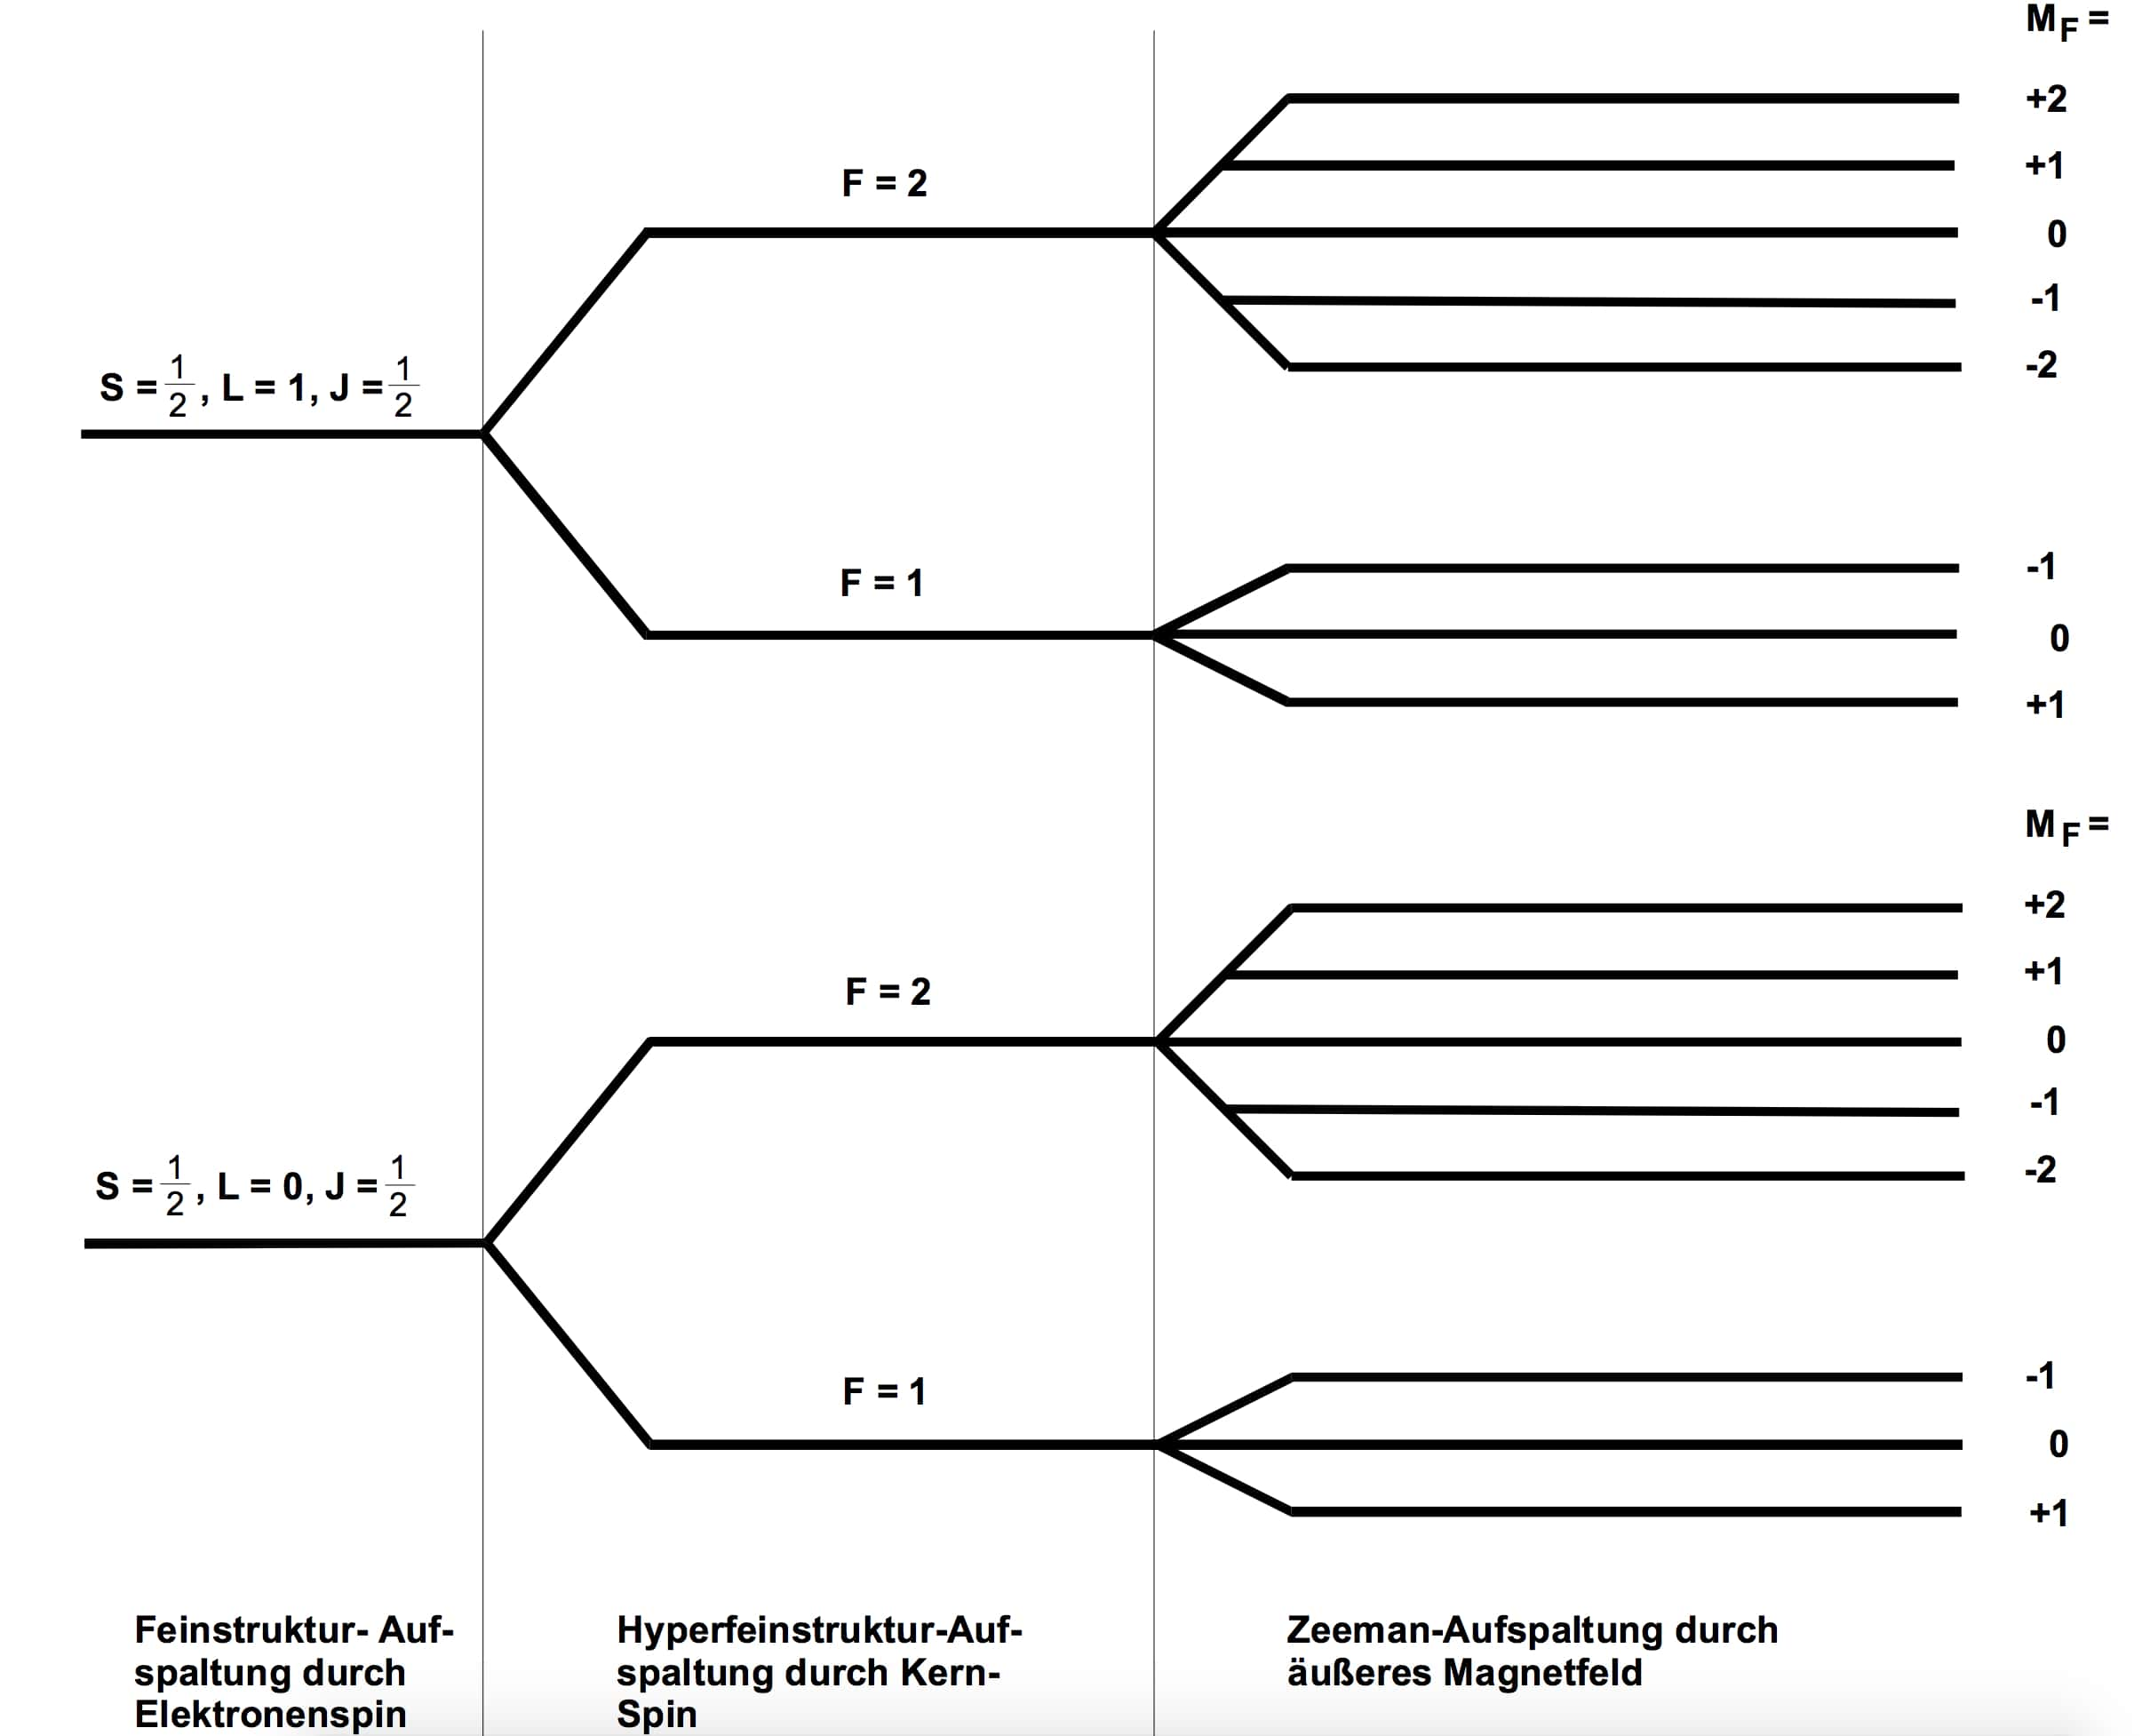
\includegraphics[width=0.8\linewidth]{img/zeemann.jpg}
	\caption{Aufspaltung der Energieniveaus durch Elektronenspin, Kernspin und Magnetfelder.}
	\label{fig:zeemann}
\end{figure}
\subsection{Optisches Pumpen}
Im Folgenden wird ein Alkali-Atom ohne Drehimpuls angenommen. Es besitz somit einen Grundzustand ${}^2\mathrm{S}_{\sfrac{1}{2}}$ und die zwei ersten angeregten Zustände ${}^2\mathrm{P}_{\sfrac{1}{2}}$ und ${}^2\mathrm{P}_{\sfrac{3}{2}}$. Die möglichen Übergänge ergeben das $\mathrm{D}_1-\mathrm{D}_2$ Dublett und sind in Abbildung \ref{fig:dublett} zu sehen.
\begin{figure}[h]
	\centering
	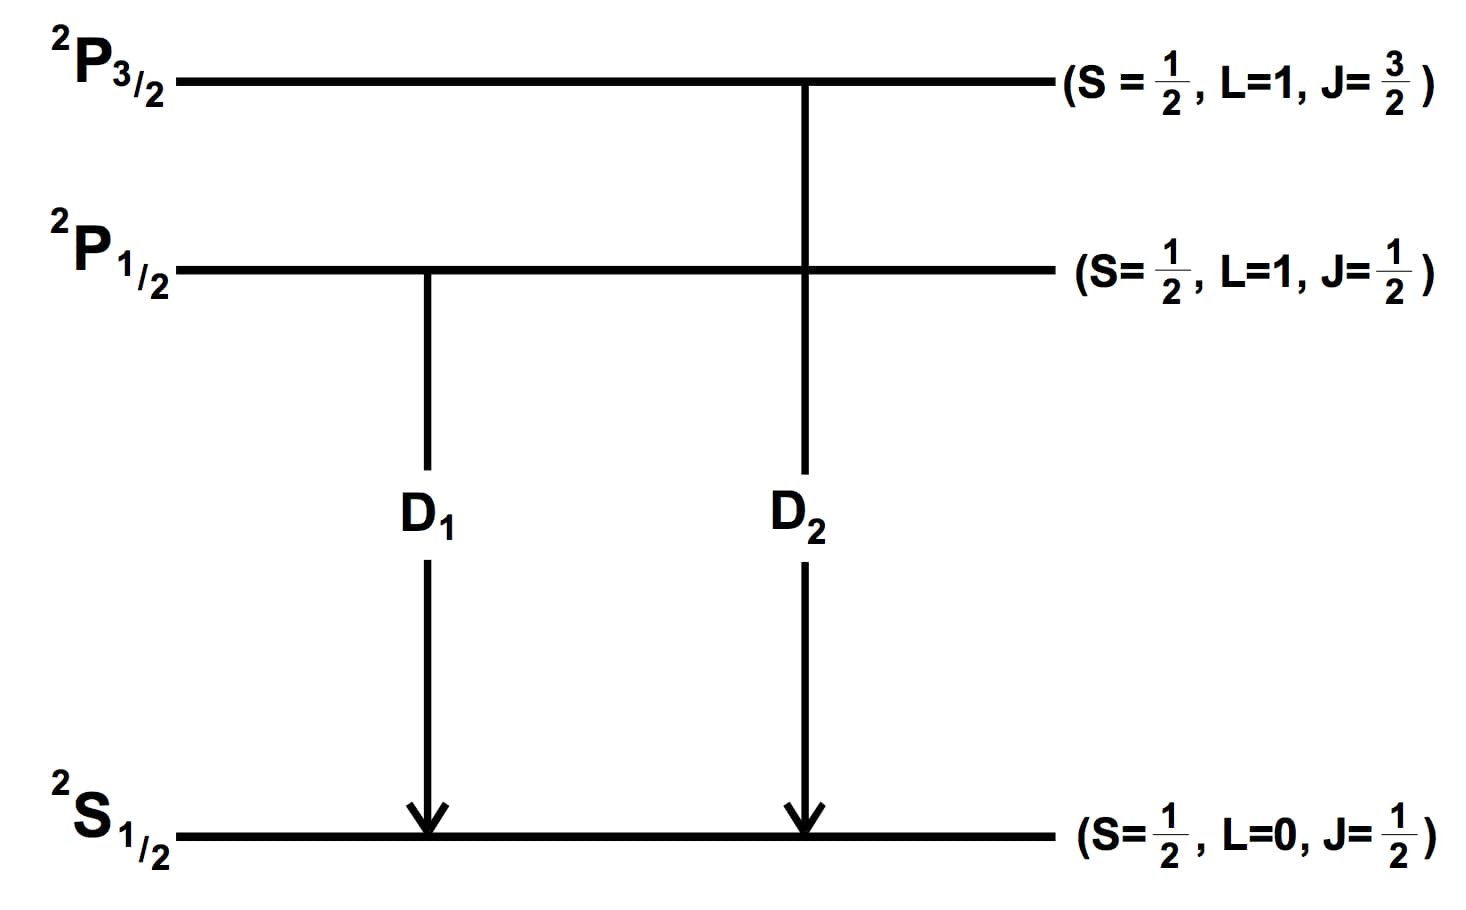
\includegraphics[width=0.8\linewidth]{img/dublett.jpg}
	\caption{Übersicht des $\mathrm{D}_1-\mathrm{D}_2$ Dublett.}
	\label{fig:dublett}
\end{figure}

In ${}^2\mathrm{S}_{\sfrac{1}{2}}$ und ${}^2\mathrm{P}_{\sfrac{1}{2}}$ ist $J={\sfrac{1}{2}}$ und daher $M_J auf \pm \sfrac{1}{2}$ beschrängt. Daraus können drei $\Delta M$ resultieren.
\begin{description}
	\item[$\Delta M=1$] Das Licht ist rechtszirkular polarisiert ($\sigma^{+}$)
	\item[$\Delta M=-1$] Das Licht ist linkszirkular polarisiert ($\sigma^{-}$)
	\item[$\Delta M=0$] Das Licht ist linear polarisiert (\pi)
\end{description}
Diese sind in Abbildung \ref{fig:ubergang} zu sehen.
\begin{figure}
	\centering
	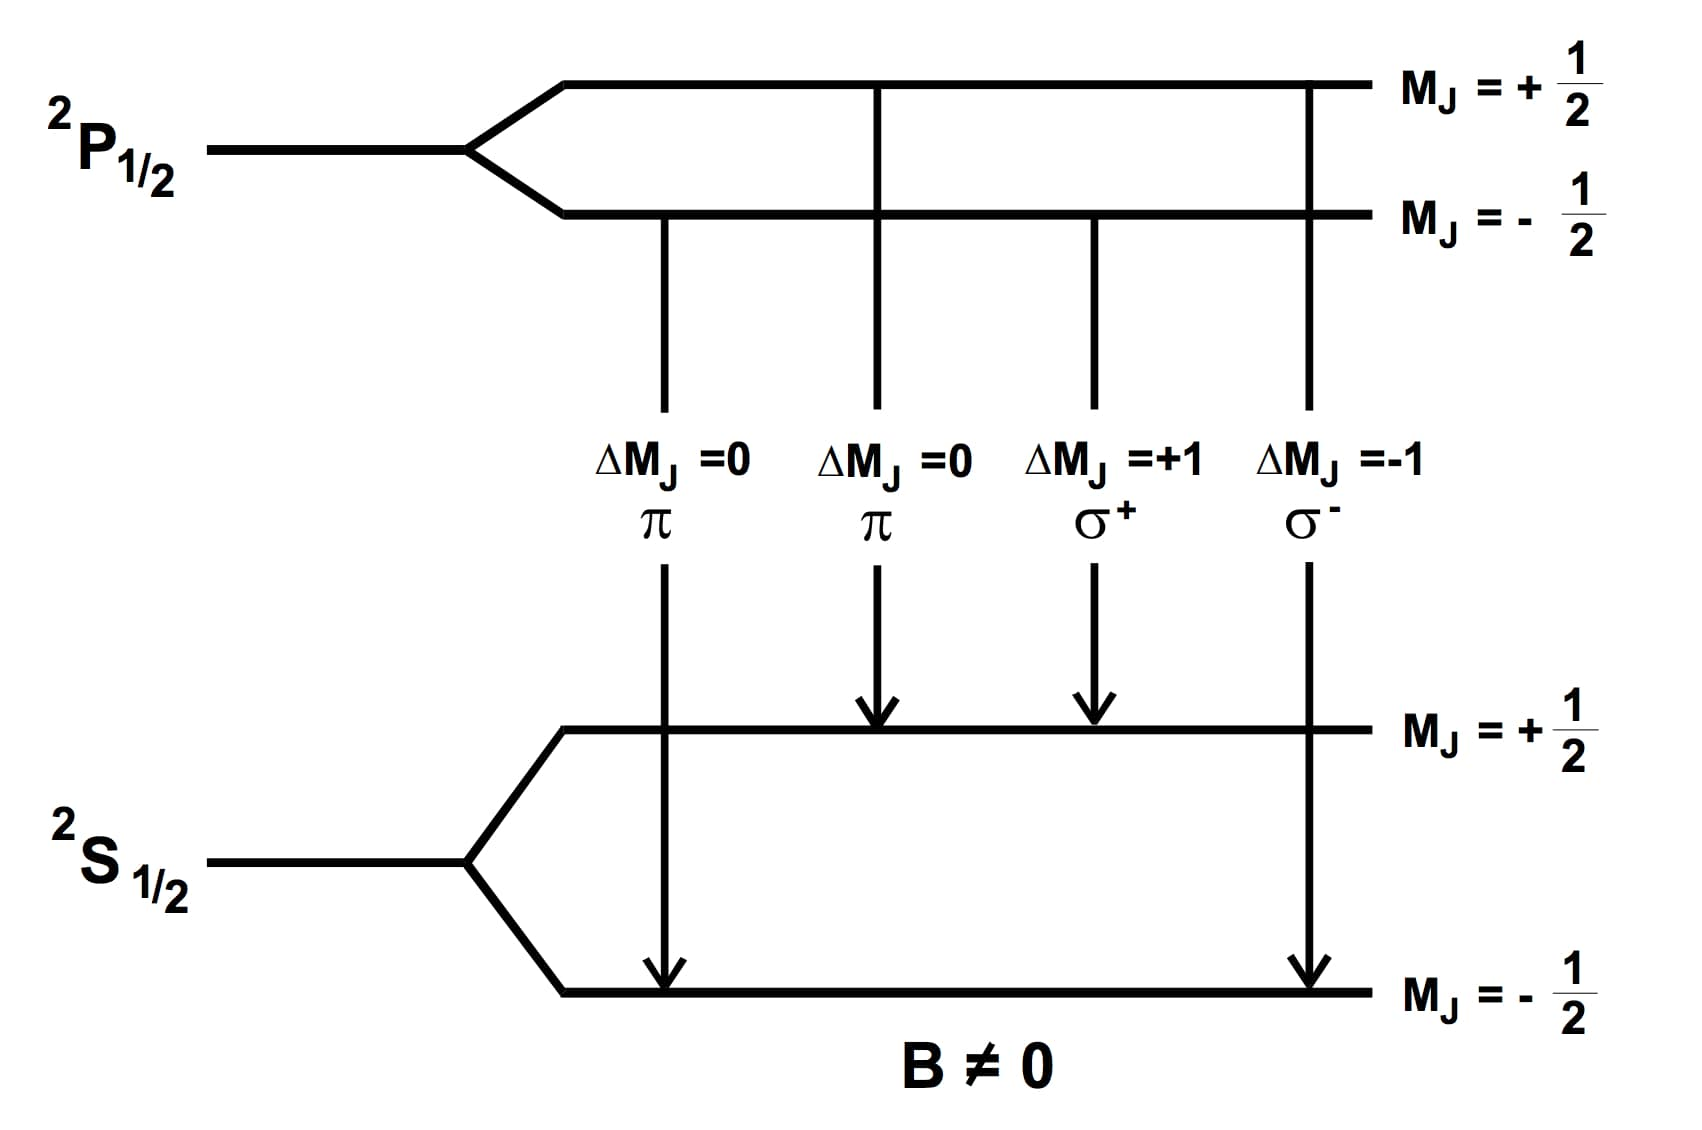
\includegraphics[width=0.8\linewidth]{img/ubergange.jpg}
	\caption{Übersicht der Übergänge für verschiedene $\Delta M$.}
	\label{fig:ubergang}
\end{figure}
Wenn nun mit rechtszirkular polarisiertes Licht angeregt wird, also $\Delta M=1$ gelten muss, ist nur der Übergang ${}^2\mathrm{S}_{\sfrac{1}{2}}, M_J=-\sfrac{1}{2}$ zu ${}^2\mathrm{P}_{\sfrac{1}{2}}, M_J=\sfrac{1}{2}$ möglich. Durch spontane Emission fallen die angeregten Elektronen dann zufällig auf die tieferen Niveaus zurück, wie in Abbildung \ref{fig:optPumpen} verdeutlicht.
\begin{figure}
	\centering
	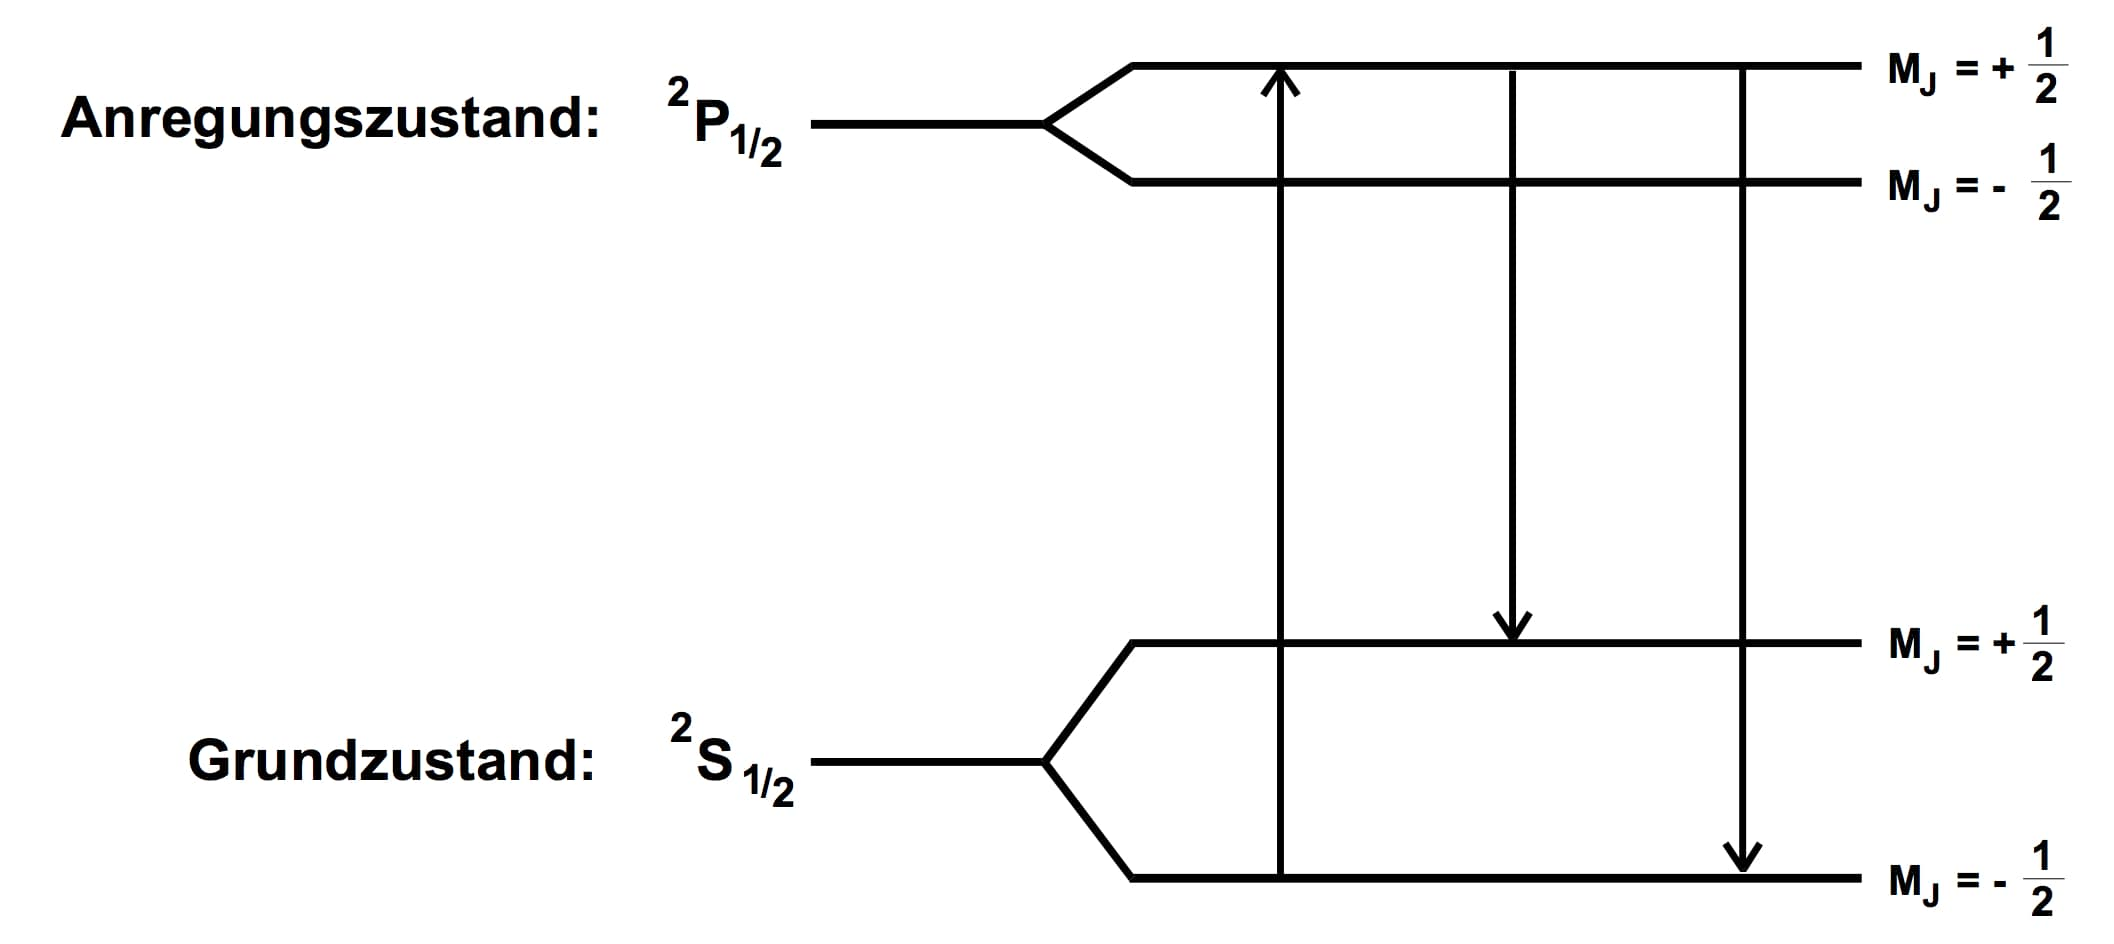
\includegraphics[width=0.8\linewidth]{img/optPumpen.jpg}
	\caption{Darstellung des optischen Pumpens.}
	\label{fig:optPumpen}
\end{figure}
Durch Wiederholung dieses Vorgangs wird ${}^2\mathrm{S}_{\sfrac{1}{2}}, M_J=-\sfrac{1}{2}$ also immer leerer und ${}^2\mathrm{S}_{\sfrac{1}{2}},M_J=\sfrac{1}{2}$ immer voller, entgegen der natürlichen Verteilung. Wenn  ${}^2\mathrm{S}_{\sfrac{1}{2}}, M_J=-\sfrac{1}{2}$ leer ist, also keine Elektronen angeregt werden können, wird kein Licht absorbiert und die Transperenz nimmt zu.
\subsection{Messung der Zeemannniveaus}
Die angeregten Elektronen können über zwei Mechanismen in einen niedrigeren Zustand über gehen. Entweder über die spontane Emission oder über die induzierte Emission. Bei der letzteren kann ein Photon, das genau die Energiedifferenz der Energieniveaus besitzt eben diesen Übergang anstoßen. Bei den in diesem Experiment untersuchten Energiedifferenzen ist die induzierte Emission die deutlich überwiegende Effekt.
\subsection{Quadratischer Zeemann-Effekt}
Für größere Magnetfelder muss ein weitere Term in die Formel \eqref{eqn:zeemann} mit aufgenommen werden. Dadurch ergibt sich:
\begin{equation}
	\Delta U_\mathrm{HF}=g_F\mu_BB + g_F^2\mu_B^2B^2\frac{1-2M_F}{\Delta E_\mathrm{Hy}}
\end{equation}
mit der Hyperfeinstrukturaufspaltung $\Delta E_{Hy}$. Es fällt auch auf, dass $U_\mathrm{HF}$ jetzt von $M_F$ abhängt.
